% Options for packages loaded elsewhere
% Options for packages loaded elsewhere
\PassOptionsToPackage{unicode}{hyperref}
\PassOptionsToPackage{hyphens}{url}
\PassOptionsToPackage{dvipsnames,svgnames,x11names}{xcolor}
%
\documentclass[
  letterpaper,
  DIV=11,
  numbers=noendperiod]{scrartcl}
\usepackage{xcolor}
\usepackage{amsmath,amssymb}
\setcounter{secnumdepth}{5}
\usepackage{iftex}
\ifPDFTeX
  \usepackage[T1]{fontenc}
  \usepackage[utf8]{inputenc}
  \usepackage{textcomp} % provide euro and other symbols
\else % if luatex or xetex
  \usepackage{unicode-math} % this also loads fontspec
  \defaultfontfeatures{Scale=MatchLowercase}
  \defaultfontfeatures[\rmfamily]{Ligatures=TeX,Scale=1}
\fi
\usepackage{lmodern}
\ifPDFTeX\else
  % xetex/luatex font selection
\fi
% Use upquote if available, for straight quotes in verbatim environments
\IfFileExists{upquote.sty}{\usepackage{upquote}}{}
\IfFileExists{microtype.sty}{% use microtype if available
  \usepackage[]{microtype}
  \UseMicrotypeSet[protrusion]{basicmath} % disable protrusion for tt fonts
}{}
\makeatletter
\@ifundefined{KOMAClassName}{% if non-KOMA class
  \IfFileExists{parskip.sty}{%
    \usepackage{parskip}
  }{% else
    \setlength{\parindent}{0pt}
    \setlength{\parskip}{6pt plus 2pt minus 1pt}}
}{% if KOMA class
  \KOMAoptions{parskip=half}}
\makeatother
% Make \paragraph and \subparagraph free-standing
\makeatletter
\ifx\paragraph\undefined\else
  \let\oldparagraph\paragraph
  \renewcommand{\paragraph}{
    \@ifstar
      \xxxParagraphStar
      \xxxParagraphNoStar
  }
  \newcommand{\xxxParagraphStar}[1]{\oldparagraph*{#1}\mbox{}}
  \newcommand{\xxxParagraphNoStar}[1]{\oldparagraph{#1}\mbox{}}
\fi
\ifx\subparagraph\undefined\else
  \let\oldsubparagraph\subparagraph
  \renewcommand{\subparagraph}{
    \@ifstar
      \xxxSubParagraphStar
      \xxxSubParagraphNoStar
  }
  \newcommand{\xxxSubParagraphStar}[1]{\oldsubparagraph*{#1}\mbox{}}
  \newcommand{\xxxSubParagraphNoStar}[1]{\oldsubparagraph{#1}\mbox{}}
\fi
\makeatother

\usepackage{color}
\usepackage{fancyvrb}
\newcommand{\VerbBar}{|}
\newcommand{\VERB}{\Verb[commandchars=\\\{\}]}
\DefineVerbatimEnvironment{Highlighting}{Verbatim}{commandchars=\\\{\}}
% Add ',fontsize=\small' for more characters per line
\usepackage{framed}
\definecolor{shadecolor}{RGB}{241,243,245}
\newenvironment{Shaded}{\begin{snugshade}}{\end{snugshade}}
\newcommand{\AlertTok}[1]{\textcolor[rgb]{0.68,0.00,0.00}{#1}}
\newcommand{\AnnotationTok}[1]{\textcolor[rgb]{0.37,0.37,0.37}{#1}}
\newcommand{\AttributeTok}[1]{\textcolor[rgb]{0.40,0.45,0.13}{#1}}
\newcommand{\BaseNTok}[1]{\textcolor[rgb]{0.68,0.00,0.00}{#1}}
\newcommand{\BuiltInTok}[1]{\textcolor[rgb]{0.00,0.23,0.31}{#1}}
\newcommand{\CharTok}[1]{\textcolor[rgb]{0.13,0.47,0.30}{#1}}
\newcommand{\CommentTok}[1]{\textcolor[rgb]{0.37,0.37,0.37}{#1}}
\newcommand{\CommentVarTok}[1]{\textcolor[rgb]{0.37,0.37,0.37}{\textit{#1}}}
\newcommand{\ConstantTok}[1]{\textcolor[rgb]{0.56,0.35,0.01}{#1}}
\newcommand{\ControlFlowTok}[1]{\textcolor[rgb]{0.00,0.23,0.31}{\textbf{#1}}}
\newcommand{\DataTypeTok}[1]{\textcolor[rgb]{0.68,0.00,0.00}{#1}}
\newcommand{\DecValTok}[1]{\textcolor[rgb]{0.68,0.00,0.00}{#1}}
\newcommand{\DocumentationTok}[1]{\textcolor[rgb]{0.37,0.37,0.37}{\textit{#1}}}
\newcommand{\ErrorTok}[1]{\textcolor[rgb]{0.68,0.00,0.00}{#1}}
\newcommand{\ExtensionTok}[1]{\textcolor[rgb]{0.00,0.23,0.31}{#1}}
\newcommand{\FloatTok}[1]{\textcolor[rgb]{0.68,0.00,0.00}{#1}}
\newcommand{\FunctionTok}[1]{\textcolor[rgb]{0.28,0.35,0.67}{#1}}
\newcommand{\ImportTok}[1]{\textcolor[rgb]{0.00,0.46,0.62}{#1}}
\newcommand{\InformationTok}[1]{\textcolor[rgb]{0.37,0.37,0.37}{#1}}
\newcommand{\KeywordTok}[1]{\textcolor[rgb]{0.00,0.23,0.31}{\textbf{#1}}}
\newcommand{\NormalTok}[1]{\textcolor[rgb]{0.00,0.23,0.31}{#1}}
\newcommand{\OperatorTok}[1]{\textcolor[rgb]{0.37,0.37,0.37}{#1}}
\newcommand{\OtherTok}[1]{\textcolor[rgb]{0.00,0.23,0.31}{#1}}
\newcommand{\PreprocessorTok}[1]{\textcolor[rgb]{0.68,0.00,0.00}{#1}}
\newcommand{\RegionMarkerTok}[1]{\textcolor[rgb]{0.00,0.23,0.31}{#1}}
\newcommand{\SpecialCharTok}[1]{\textcolor[rgb]{0.37,0.37,0.37}{#1}}
\newcommand{\SpecialStringTok}[1]{\textcolor[rgb]{0.13,0.47,0.30}{#1}}
\newcommand{\StringTok}[1]{\textcolor[rgb]{0.13,0.47,0.30}{#1}}
\newcommand{\VariableTok}[1]{\textcolor[rgb]{0.07,0.07,0.07}{#1}}
\newcommand{\VerbatimStringTok}[1]{\textcolor[rgb]{0.13,0.47,0.30}{#1}}
\newcommand{\WarningTok}[1]{\textcolor[rgb]{0.37,0.37,0.37}{\textit{#1}}}

\usepackage{longtable,booktabs,array}
\usepackage{calc} % for calculating minipage widths
% Correct order of tables after \paragraph or \subparagraph
\usepackage{etoolbox}
\makeatletter
\patchcmd\longtable{\par}{\if@noskipsec\mbox{}\fi\par}{}{}
\makeatother
% Allow footnotes in longtable head/foot
\IfFileExists{footnotehyper.sty}{\usepackage{footnotehyper}}{\usepackage{footnote}}
\makesavenoteenv{longtable}
\usepackage{graphicx}
\makeatletter
\newsavebox\pandoc@box
\newcommand*\pandocbounded[1]{% scales image to fit in text height/width
  \sbox\pandoc@box{#1}%
  \Gscale@div\@tempa{\textheight}{\dimexpr\ht\pandoc@box+\dp\pandoc@box\relax}%
  \Gscale@div\@tempb{\linewidth}{\wd\pandoc@box}%
  \ifdim\@tempb\p@<\@tempa\p@\let\@tempa\@tempb\fi% select the smaller of both
  \ifdim\@tempa\p@<\p@\scalebox{\@tempa}{\usebox\pandoc@box}%
  \else\usebox{\pandoc@box}%
  \fi%
}
% Set default figure placement to htbp
\def\fps@figure{htbp}
\makeatother





\setlength{\emergencystretch}{3em} % prevent overfull lines

\providecommand{\tightlist}{%
  \setlength{\itemsep}{0pt}\setlength{\parskip}{0pt}}



 


\KOMAoption{captions}{tableheading}
\makeatletter
\@ifpackageloaded{caption}{}{\usepackage{caption}}
\AtBeginDocument{%
\ifdefined\contentsname
  \renewcommand*\contentsname{Table of contents}
\else
  \newcommand\contentsname{Table of contents}
\fi
\ifdefined\listfigurename
  \renewcommand*\listfigurename{List of Figures}
\else
  \newcommand\listfigurename{List of Figures}
\fi
\ifdefined\listtablename
  \renewcommand*\listtablename{List of Tables}
\else
  \newcommand\listtablename{List of Tables}
\fi
\ifdefined\figurename
  \renewcommand*\figurename{Figure}
\else
  \newcommand\figurename{Figure}
\fi
\ifdefined\tablename
  \renewcommand*\tablename{Table}
\else
  \newcommand\tablename{Table}
\fi
}
\@ifpackageloaded{float}{}{\usepackage{float}}
\floatstyle{ruled}
\@ifundefined{c@chapter}{\newfloat{codelisting}{h}{lop}}{\newfloat{codelisting}{h}{lop}[chapter]}
\floatname{codelisting}{Listing}
\newcommand*\listoflistings{\listof{codelisting}{List of Listings}}
\makeatother
\makeatletter
\makeatother
\makeatletter
\@ifpackageloaded{caption}{}{\usepackage{caption}}
\@ifpackageloaded{subcaption}{}{\usepackage{subcaption}}
\makeatother
\usepackage{bookmark}
\IfFileExists{xurl.sty}{\usepackage{xurl}}{} % add URL line breaks if available
\urlstyle{same}
\hypersetup{
  pdftitle={STAT 211: Normal Distribution},
  colorlinks=true,
  linkcolor={blue},
  filecolor={Maroon},
  citecolor={Blue},
  urlcolor={Blue},
  pdfcreator={LaTeX via pandoc}}


\title{STAT 211: Normal Distribution}
\usepackage{etoolbox}
\makeatletter
\providecommand{\subtitle}[1]{% add subtitle to \maketitle
  \apptocmd{\@title}{\par {\large #1 \par}}{}{}
}
\makeatother
\subtitle{Computing probabilities and quantiles from this important
distribution}
\author{}
\date{}
\begin{document}
\maketitle

\renewcommand*\contentsname{Table of contents}
{
\hypersetup{linkcolor=}
\setcounter{tocdepth}{3}
\tableofcontents
}

\begin{verbatim}
Loading required package: ggplot2
\end{verbatim}

\section{The Normal Distribution}\label{the-normal-distribution}

\subsection{Defining the normal
distribution}\label{defining-the-normal-distribution}

The {normal} (also known as `Gaussian') is \(X\sim N(\mu,\sigma^2)\):

\begin{itemize}
\tightlist
\item
  \(\mu\) is the expected value (\(E[X]\))
\item
  \(\sigma^2\) is the variance of (\(Var[X]\))
\end{itemize}

Its pdf:

\[ 
f(x)=\frac1{(2\pi\sigma^2)^{1/2}}e^{-\frac{(x-\mu)^2}{2\sigma^2}} 
\]

{(Just like the binomial, you don't need to know this formula for this
class)}

\subsection{Computing probabilities: old
vs.~new}\label{computing-probabilities-old-vs.-new}

Computing probabilities with the normal \textbf{requires} computers

In times of yore, this meant using tables:

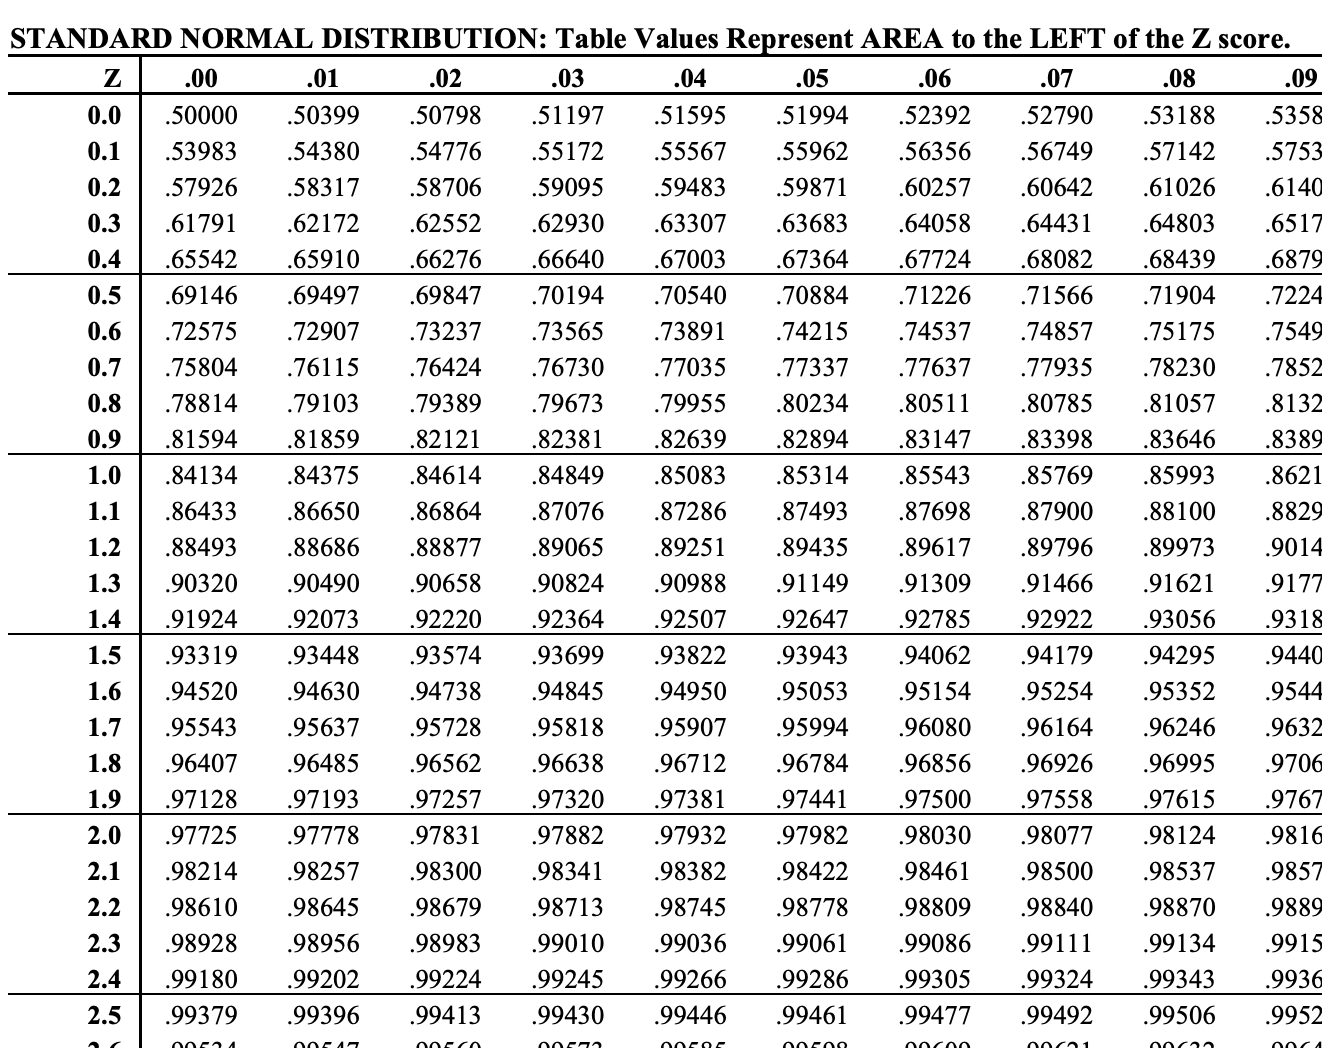
\includegraphics[width=3.5\linewidth,height=\textheight,keepaspectratio]{figures/normalTable.png}

Now, we can just use a computer:

\begin{Shaded}
\begin{Highlighting}[]
\FunctionTok{pnorm}\NormalTok{(}\FloatTok{1.8}\NormalTok{,}\DecValTok{0}\NormalTok{,}\DecValTok{1}\NormalTok{)}
\end{Highlighting}
\end{Shaded}

\begin{verbatim}
[1] 0.9640697
\end{verbatim}

\begin{Shaded}
\begin{Highlighting}[]
\FunctionTok{pnorm}\NormalTok{(}\FloatTok{1.89}\NormalTok{,}\DecValTok{0}\NormalTok{,}\DecValTok{1}\NormalTok{)}
\end{Highlighting}
\end{Shaded}

\begin{verbatim}
[1] 0.970621
\end{verbatim}

\section{Computing Probabilities and
Values}\label{computing-probabilities-and-values}

\subsection{Computing probabilities}\label{computing-probabilities}

We will always write \(X\sim N(\mu,\sigma^2)\) for the normal

R syntax will be specified with \(\mu\) and \(\sigma = \sqrt{\sigma^2}\)
instead

{Example}

If \(X \sim N(5,9)\), then the probability \(X\) is less than 4 is:

\begin{Shaded}
\begin{Highlighting}[numbers=left,,]
\NormalTok{x       }\OtherTok{=} \DecValTok{4}
\NormalTok{mu      }\OtherTok{=} \DecValTok{5}
\NormalTok{sigmaSq }\OtherTok{=} \DecValTok{9}
\FunctionTok{pnorm}\NormalTok{(x, mu, }\FunctionTok{sqrt}\NormalTok{(sigmaSq))}
\end{Highlighting}
\end{Shaded}

\begin{verbatim}
[1] 0.3694413
\end{verbatim}

\subsection{Computing values
(quantiles)}\label{computing-values-quantiles}

Continuing with \(X \sim N(5,9)\):

{(that is, normal with expected value 5 and variance 9)}

{Recall:}

For a value \(x = 4\), \(P(X \leq 4)\):

\begin{Shaded}
\begin{Highlighting}[]
\FunctionTok{pnorm}\NormalTok{(}\DecValTok{4}\NormalTok{,}\DecValTok{5}\NormalTok{,}\DecValTok{3}\NormalTok{)}
\end{Highlighting}
\end{Shaded}

\begin{verbatim}
[1] 0.3694413
\end{verbatim}

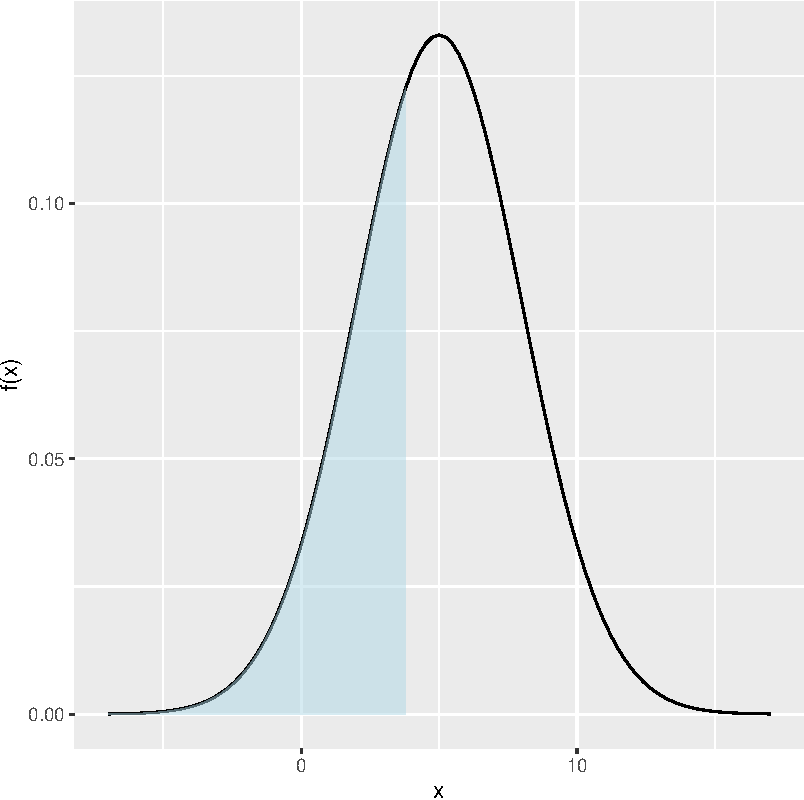
\includegraphics[width=1\linewidth,height=\textheight,keepaspectratio]{chapter3normal_files/figure-pdf/normalProbPlot-1.pdf}

Now, let's ask the \textbf{opposite} question!

For a fixed probability \(p\), what is the value \(x\) so that
\(P(X \leq x) = p\)?

This value is called a {quantile}

{Example:}

What \(x\) makes \(P(X\leq x) = .7\)?

\begin{Shaded}
\begin{Highlighting}[]
\FunctionTok{qnorm}\NormalTok{(.}\DecValTok{7}\NormalTok{,}\DecValTok{5}\NormalTok{,}\DecValTok{3}\NormalTok{)}
\end{Highlighting}
\end{Shaded}

\begin{verbatim}
[1] 6.573202
\end{verbatim}

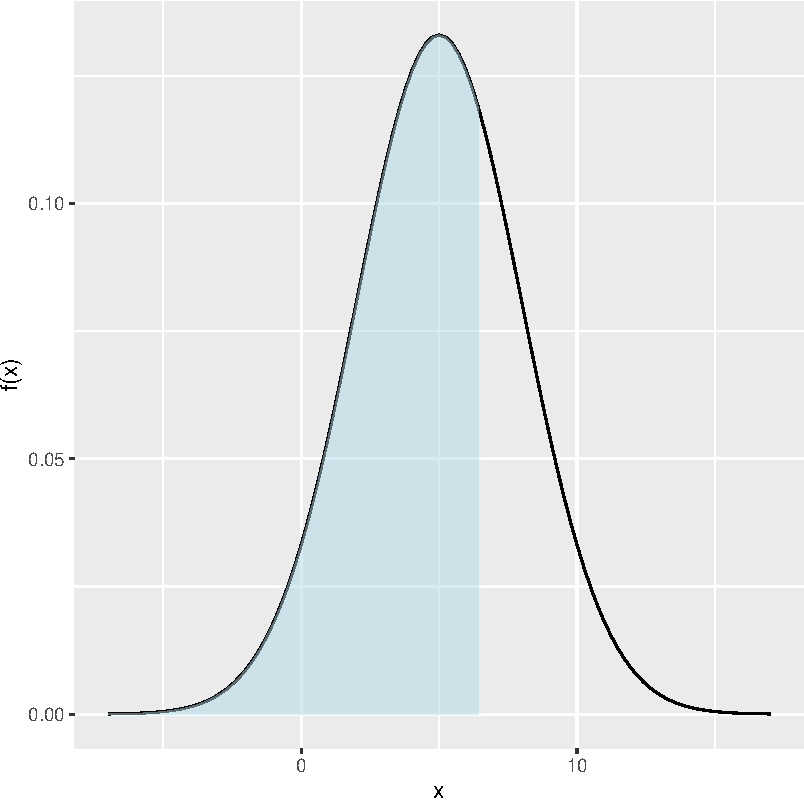
\includegraphics[width=1\linewidth,height=\textheight,keepaspectratio]{chapter3normal_files/figure-pdf/normalQuantilePlot-1.pdf}

\subsection{Using pnorm and qnorm}\label{using-pnorm-and-qnorm}

{Concept Check:} What would each of the following codes produce?

\begin{Shaded}
\begin{Highlighting}[]
\FunctionTok{qnorm}\NormalTok{( }\FunctionTok{pnorm}\NormalTok{(}\DecValTok{3}\NormalTok{,}\DecValTok{5}\NormalTok{,}\DecValTok{3}\NormalTok{), }\DecValTok{5}\NormalTok{, }\DecValTok{3}\NormalTok{)}
\end{Highlighting}
\end{Shaded}

. . .

\begin{verbatim}
[1] 3
\end{verbatim}

. . .

\begin{Shaded}
\begin{Highlighting}[]
\FunctionTok{pnorm}\NormalTok{( }\FunctionTok{qnorm}\NormalTok{(.}\DecValTok{2}\NormalTok{,}\DecValTok{5}\NormalTok{,}\DecValTok{3}\NormalTok{), }\DecValTok{5}\NormalTok{, }\DecValTok{3}\NormalTok{)}
\end{Highlighting}
\end{Shaded}

. . .

\begin{verbatim}
[1] 0.2
\end{verbatim}

\subsection{Computing probabilities and
values}\label{computing-probabilities-and-values-1}

Suppose \(X \sim N(-3.2, 100)\)

{that is, normal with expected value -3.2 and variance 100}

{Probability:} What is the probability \(X\) equals 0?

. . .

This is always zero!

. . .

{Probability:} What is the probability \(X\) is less than 0?

. . .

\begin{Shaded}
\begin{Highlighting}[]
\FunctionTok{pnorm}\NormalTok{(}\DecValTok{0}\NormalTok{,}\SpecialCharTok{{-}}\FloatTok{3.2}\NormalTok{,}\FunctionTok{sqrt}\NormalTok{(}\DecValTok{100}\NormalTok{))}
\end{Highlighting}
\end{Shaded}

\begin{verbatim}
[1] 0.6255158
\end{verbatim}

. . .

{Values:} at what value \(x\) does \(P(X\leq x) = .05\)?

. . .

\begin{Shaded}
\begin{Highlighting}[]
\FunctionTok{qnorm}\NormalTok{(.}\DecValTok{05}\NormalTok{,}\SpecialCharTok{{-}}\FloatTok{3.2}\NormalTok{,}\FunctionTok{sqrt}\NormalTok{(}\DecValTok{100}\NormalTok{))}
\end{Highlighting}
\end{Shaded}

\begin{verbatim}
[1] -19.64854
\end{verbatim}

\subsection{Computing probabilities:
SATs}\label{computing-probabilities-sats}

{Example}

The scores on the SAT math section are \(X \sim N(520,3600)\)

{(that is, normal with expected value 520 and variance 3600)}

What is the probability someone scores less than 600?

\(P(X \leq 600) = \text{what probability?}\)

\begin{Shaded}
\begin{Highlighting}[]
\NormalTok{x       }\OtherTok{=} \DecValTok{600}
\NormalTok{mu      }\OtherTok{=} \DecValTok{520}
\NormalTok{sigmaSq }\OtherTok{=} \DecValTok{3600}
\FunctionTok{pnorm}\NormalTok{(x, mu, }\FunctionTok{sqrt}\NormalTok{(sigmaSq))}
\end{Highlighting}
\end{Shaded}

\begin{verbatim}
[1] 0.9087888
\end{verbatim}

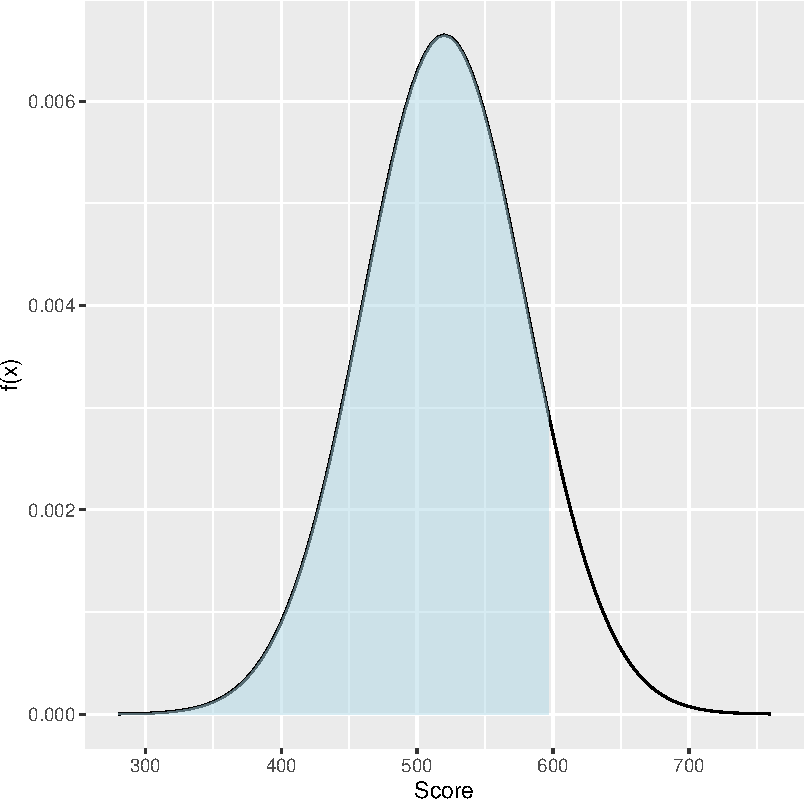
\includegraphics[width=1.2\linewidth,height=\textheight,keepaspectratio]{chapter3normal_files/figure-pdf/SATprobabilityNoEcho-1.pdf}

\subsection{Computing values: SATs}\label{computing-values-sats}

{Example}

The scores on the SAT math section are \(X \sim N(520,3600)\)

The stats dept. admits students scoring above \(96^{th}\) percentile

What is the cutoff score (\(x\)) for recruitment by the stats dept.?

\(P(X \leq x) = 0.96\)

\begin{Shaded}
\begin{Highlighting}[]
\NormalTok{prob    }\OtherTok{=}\NormalTok{ .}\DecValTok{96}
\NormalTok{mu      }\OtherTok{=} \DecValTok{520}
\NormalTok{sigmaSq }\OtherTok{=} \DecValTok{3600}
\FunctionTok{qnorm}\NormalTok{(prob, mu, }\FunctionTok{sqrt}\NormalTok{(sigmaSq))}
\end{Highlighting}
\end{Shaded}

\begin{verbatim}
[1] 625.0412
\end{verbatim}

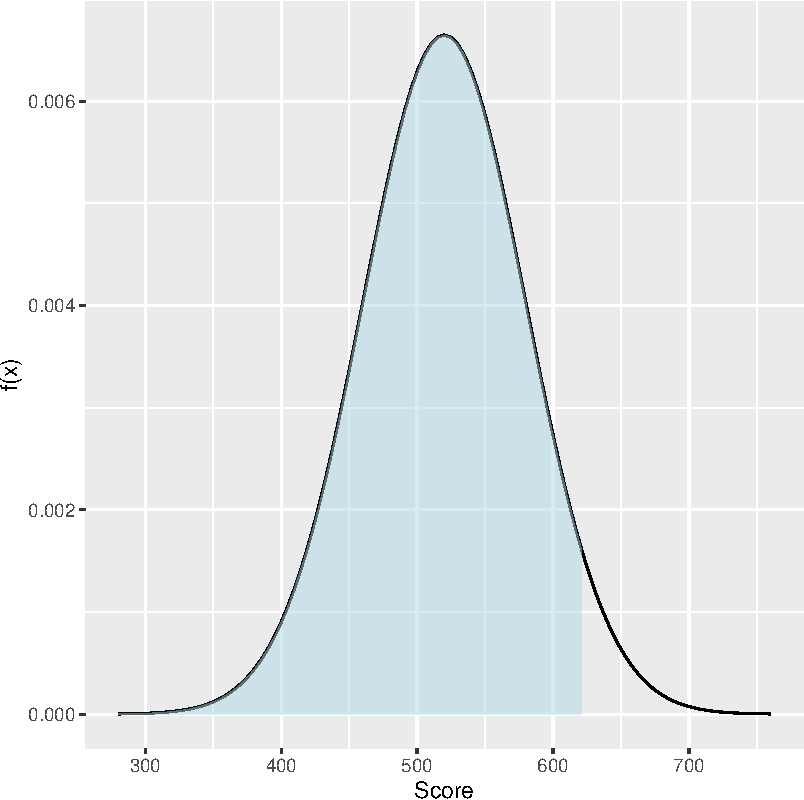
\includegraphics[width=1\linewidth,height=\textheight,keepaspectratio]{chapter3normal_files/figure-pdf/SATvalueNoEcho-1.pdf}

\section{Transformations}\label{transformations}

\subsection{\texorpdfstring{Transforming Normals:
\(aX + b\)}{Transforming Normals: aX + b}}\label{transformingNormals}

Suppose again \(X \sim N(\mu, \sigma^2)\)

If we multiply/add constants \(a,b\) to \(X\) to form a new rv \(Y\):

\[
Y  = aX + b 
\]

then \(Y \sim N(a\mu + b, a^2 \sigma^2)\)

{(This should remind you of our \(E[X]\) and \(Var[X]\) results)}

{Example:}

If \(X \sim N(150,100)\) then

\[
Y = 3X + 30 \sim N(480, 900)
\]

\subsection{Transforming Normals: inches to
cm}\label{transforming-normals-inches-to-cm}

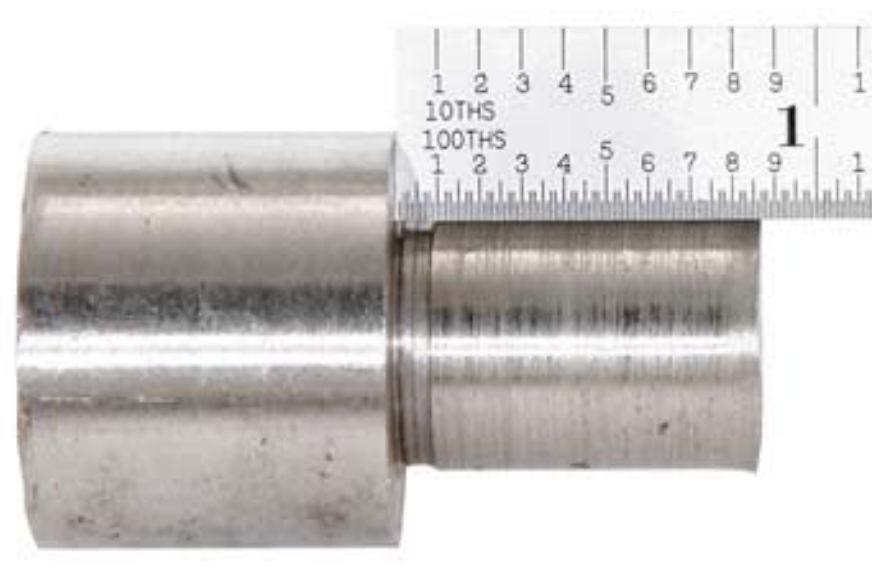
\includegraphics[width=0.5\linewidth,height=\textheight,keepaspectratio]{figures/steelRuler.png}

We are measuring a machined part using a ruler on a .01'' scale

If several people measure, they will get some random amount of
measurement error:

\[
X \sim N(.875, .00005)
\]

What is the probability that that a measurement will be within
\(\pm\).01 centimeters?

{(An inch is 2.54 cm)}

\(Y = 2.54X\), therefore
\(Y \sim N(2.54*.875,  2.54^2*.00005) = N(2.2225,  0.00032)\)

\[
\begin{align}
P(2.2225 - .01 \leq Y \leq 2.2225 + .01) & = \\
 = P(2.2125 \leq Y \leq 2.2325) & \\
 = F(2.2325) - F(2.2125)
\end{align}
\]

\begin{Shaded}
\begin{Highlighting}[]
\NormalTok{mu      }\OtherTok{=} \FloatTok{2.54}\SpecialCharTok{*}\NormalTok{.}\DecValTok{875}
\NormalTok{sigmaSq }\OtherTok{=} \FloatTok{2.54}\SpecialCharTok{\^{}}\DecValTok{2}\SpecialCharTok{*}\NormalTok{.}\DecValTok{00005}
\FunctionTok{pnorm}\NormalTok{(mu }\SpecialCharTok{+}\NormalTok{ .}\DecValTok{01}\NormalTok{, mu, }\FunctionTok{sqrt}\NormalTok{(sigmaSq)) }\SpecialCharTok{{-}} 
    \FunctionTok{pnorm}\NormalTok{(mu }\SpecialCharTok{{-}}\NormalTok{ .}\DecValTok{01}\NormalTok{, mu, }\FunctionTok{sqrt}\NormalTok{(sigmaSq))}
\end{Highlighting}
\end{Shaded}

\begin{verbatim}
[1] 0.4223202
\end{verbatim}

\subsection{The Standard Normal
Distribution}\label{the-standard-normal-distribution}

When \(\mu=0\) and \(\sigma=1\), we call it the {standard normal}

\[
f(x)=\frac1{\sqrt{2\pi}}e^{-x^2/2},\,\,-\infty<x<\infty.
\]

{(Once again, you don't need to know this formula for this class)}

The standard normal will be notated as: \(Z \sim N(0,1)\)

\subsection{Standardization}\label{standardization}

Going from a general normal to a standard normal is known as
{standardization}

\[
X \sim N(\mu, \sigma^2) \longrightarrow Z = \frac{X - \mu}{\sigma} \sim N(0,1)
\]

The opposite (actually, the {inverse}) is true

\[
Z \sim N(0, 1) \longrightarrow X = Z \sigma + \mu \sim N(\mu,\sigma^2)
\]

{(this is using the results in
\hyperref[transformingNormals]{Transforming Normals})}

\section{Z-scores: How to compare
values}\label{z-scores-how-to-compare-values}

\subsection{Z-scores: Comparing values}\label{z-scores-comparing-values}

The {z-score} can be computed:

\[
\text{z-score} = \frac{x - \mu}{\sigma}
\]

{(For a value \(x\) from a distribution with mean \(\mu\) and variance
\(\sigma^2\))}

{Question:} Which of the two values from two different distributions is
more {unusual}?

{Answer:} Whichever z-score has larger {magnitude}

{(that is, largest \textbar z-score\textbar)}

{Example:} We want to compare olympic records in men's and women's
sprinting. Which is more unusual?

Let's look at a table:

\begin{longtable}[]{@{}lrr@{}}
\caption{Table of Average and Standard Deviation of Olympic Sprinting
times.}\tabularnewline
\toprule\noalign{}
Category & Mens & Womens \\
\midrule\noalign{}
\endfirsthead
\toprule\noalign{}
Category & Mens & Womens \\
\midrule\noalign{}
\endhead
\bottomrule\noalign{}
\endlastfoot
average & 9.85 & 10.83 \\
variance & .0057 & .0049 \\
record & 9.63 & 10.61 \\
\end{longtable}

Let's compute the two {z-scores}:

\begin{Shaded}
\begin{Highlighting}[]
\NormalTok{zScoreM }\OtherTok{=}\NormalTok{ (}\FloatTok{9.63} \SpecialCharTok{{-}} \FloatTok{9.85}\NormalTok{)}\SpecialCharTok{/}\FunctionTok{sqrt}\NormalTok{(.}\DecValTok{0057}\NormalTok{)}
\NormalTok{zScoreM}
\end{Highlighting}
\end{Shaded}

\begin{verbatim}
[1] -2.913971
\end{verbatim}

\begin{Shaded}
\begin{Highlighting}[]
\NormalTok{zScoreW }\OtherTok{=}\NormalTok{ (}\FloatTok{10.61} \SpecialCharTok{{-}} \FloatTok{10.83}\NormalTok{)}\SpecialCharTok{/}\FunctionTok{sqrt}\NormalTok{(.}\DecValTok{0049}\NormalTok{)}
\NormalTok{zScoreW}
\end{Highlighting}
\end{Shaded}

\begin{verbatim}
[1] -3.142857
\end{verbatim}

The women's result is more unusual

The z-score for men is -2.914 while for women it is -3.143

\subsection{Z-scores: Another
application}\label{z-scores-another-application}

Another use of {z-scores}: what value \(x\) would be equally as unusual?

{Answer:} Choose the \(x\) so that the z-scores are {equal}

{Example:} What time for a men's sprinter would be equivalent to the
female record?

\begin{longtable}[]{@{}lrr@{}}
\caption{Table of Average and Standard Deviation of Olympic Sprinting
times.}\tabularnewline
\toprule\noalign{}
Category & Mens & Womens \\
\midrule\noalign{}
\endfirsthead
\toprule\noalign{}
Category & Mens & Womens \\
\midrule\noalign{}
\endhead
\bottomrule\noalign{}
\endlastfoot
average & 9.85 & 10.83 \\
variance & .0057 & .0049 \\
record & 9.63 & 10.61 \\
\end{longtable}

We found the female z-score = \(\frac{10.61 - 10.83}{\sqrt{.0049}}\) =
-3.143

To find the equivalent time, we need to {unstandardize} \[
\text{z-score}*\sigma  + \mu = x
\]

Here, use

\begin{itemize}
\tightlist
\item
  z-score from the female sprinters
\item
  the \(\mu\) and \(\sigma\) from the male sprinters (\(\mu = 9.85\),
  \(\sigma^2 = .0057\))
\end{itemize}

\begin{Shaded}
\begin{Highlighting}[]
\NormalTok{x }\OtherTok{=}\NormalTok{ zScoreW }\SpecialCharTok{*} \FunctionTok{sqrt}\NormalTok{(.}\DecValTok{0057}\NormalTok{) }\SpecialCharTok{+} \FloatTok{9.85}
\NormalTok{x}
\end{Highlighting}
\end{Shaded}

\begin{verbatim}
[1] 9.612719
\end{verbatim}

The male record would need to be 9.613 seconds to be as unusual as the
female record.

\subsection{Empirical rule}\label{empirical-rule}

Values from normal distributions contain predictable amounts of
probability

This is the {empirical rule:}

\begin{itemize}
\tightlist
\item
  {\(P( |Z| \leq 1) = 0.683\)} (\(\sim \frac{2}{3}\) obs. within 1
  \(\sigma\))
\item
  {\(P( |Z| \leq 2) = 0.954\)} (\(\sim \frac{19}{20}\) obs. within 2
  \(\sigma\))
\item
  {\(P( |Z| \leq 3) = 0.997\)} (\(\sim \frac{99}{100}\) obs. within 3
  \(\sigma\))
\end{itemize}

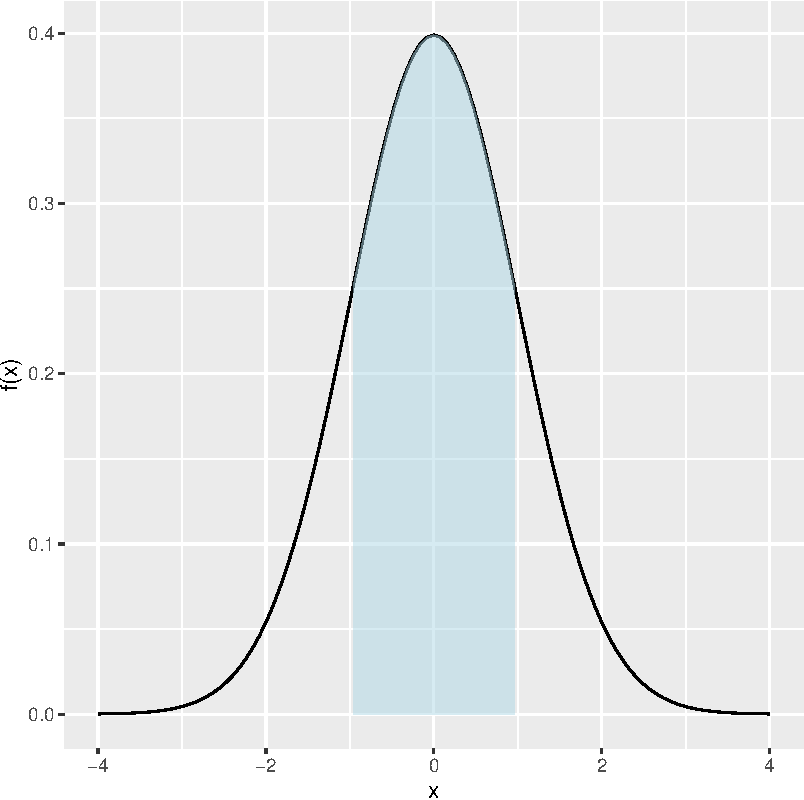
\includegraphics[width=1.1\linewidth,height=\textheight,keepaspectratio]{chapter3normal_files/figure-pdf/normalEmpRuleGeneral1-1.pdf}

{\(P( |Z| \leq 1) = 0.68\)}

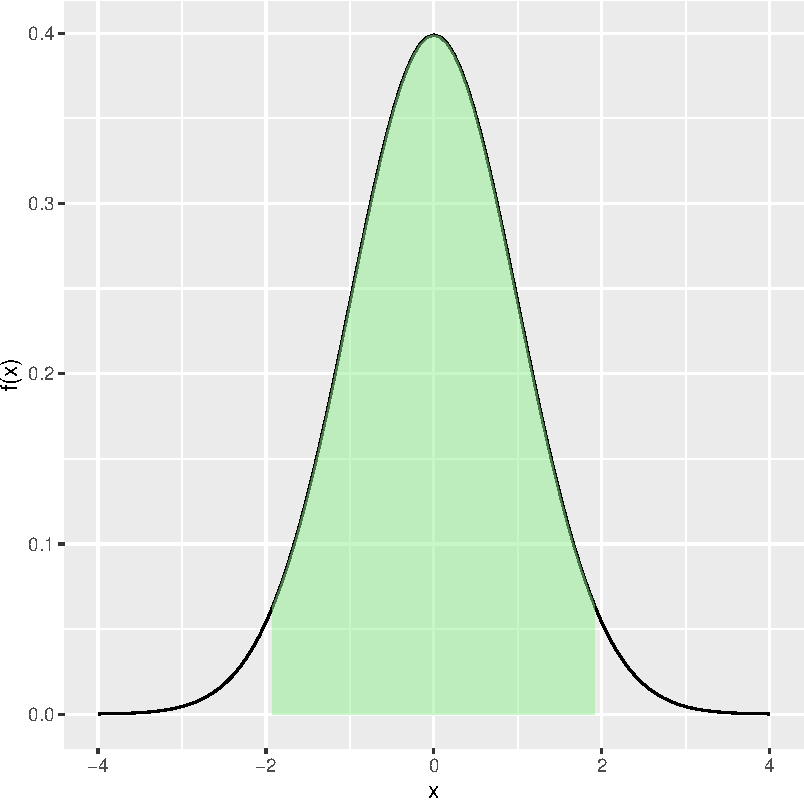
\includegraphics[width=1.1\linewidth,height=\textheight,keepaspectratio]{chapter3normal_files/figure-pdf/normalEmpRuleGeneral2-1.pdf}

{\(P( |Z| \leq 2) = 0.95\)}

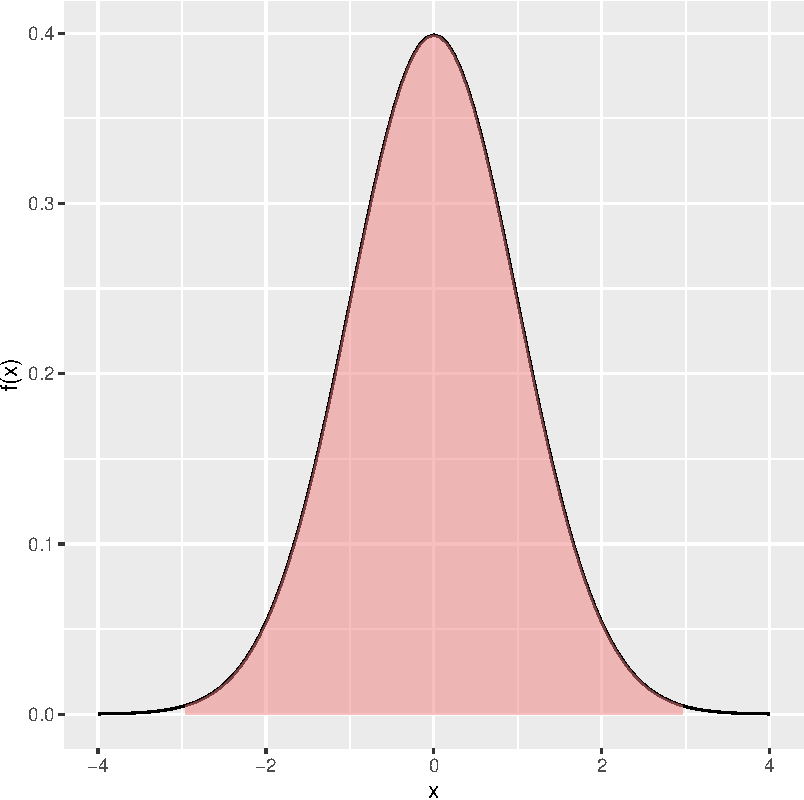
\includegraphics[width=1.1\linewidth,height=\textheight,keepaspectratio]{chapter3normal_files/figure-pdf/normalEmpRuleGeneral3-1.pdf}

{\(P( |Z| \leq 3) = 0.997\)}

\subsection{A (potentially) helpful
applet}\label{a-potentially-helpful-applet}

On exams, there will be a link to an applet:
\href{https://people.tamu.edu/~scottcrawford/ftable.html}{Probability
applet}

{Note: This applet is totally optional and unnecessary if you use R}

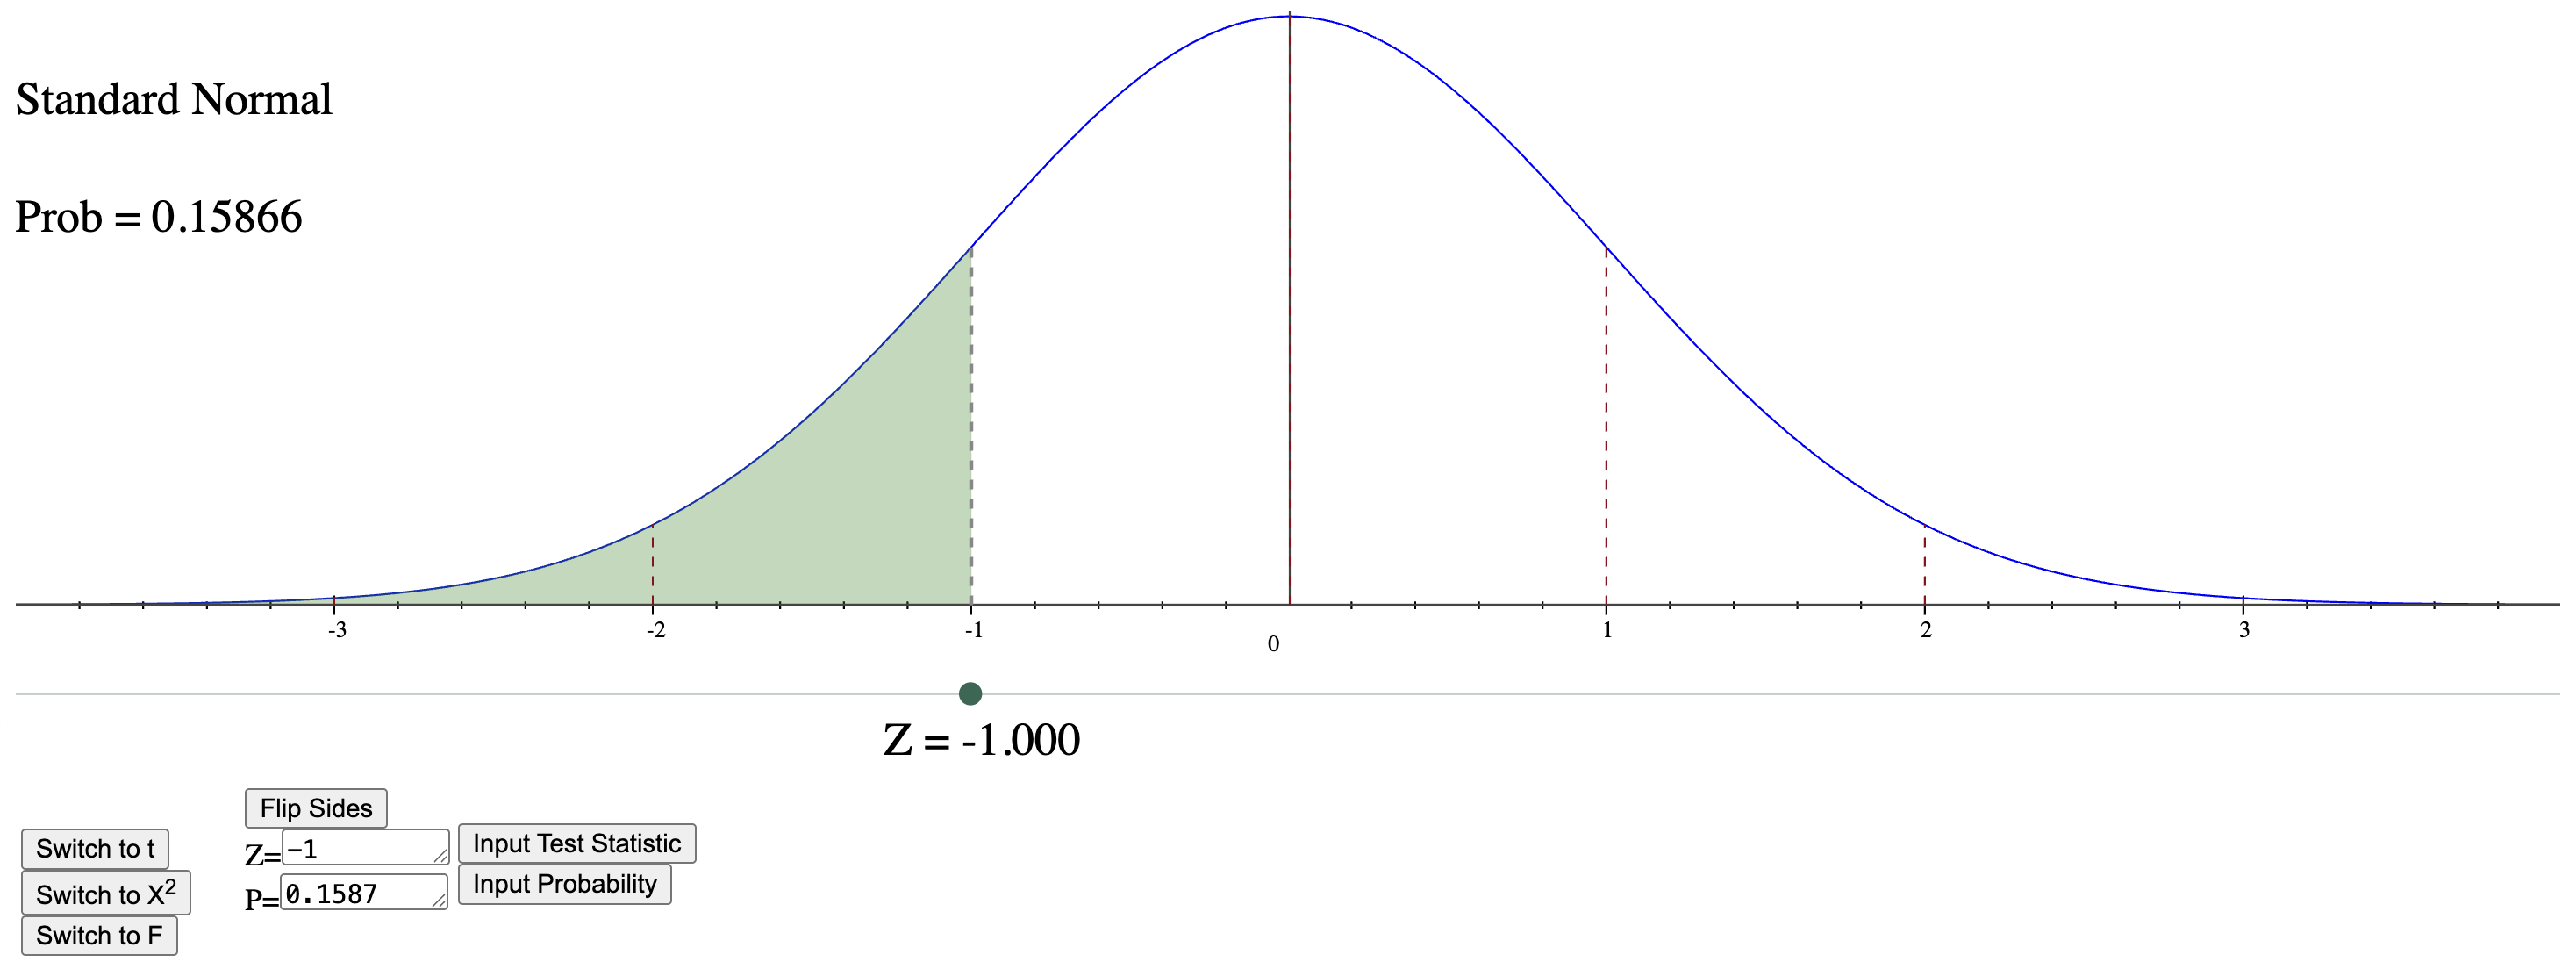
\includegraphics[width=7.29167in,height=\textheight,keepaspectratio]{figures/appletScott.png}

Returning to SAT example:

\begin{Shaded}
\begin{Highlighting}[]
\NormalTok{x       }\OtherTok{=} \DecValTok{600}
\NormalTok{mu      }\OtherTok{=} \DecValTok{520}
\NormalTok{sigmaSq }\OtherTok{=} \DecValTok{3600}
\FunctionTok{pnorm}\NormalTok{(x, mu, }\FunctionTok{sqrt}\NormalTok{(sigmaSq))}
\end{Highlighting}
\end{Shaded}

\begin{verbatim}
[1] 0.9087888
\end{verbatim}

\begin{Shaded}
\begin{Highlighting}[]
\FunctionTok{qnorm}\NormalTok{(.}\DecValTok{96}\NormalTok{, mu, }\FunctionTok{sqrt}\NormalTok{(sigmaSq))}
\end{Highlighting}
\end{Shaded}

\begin{verbatim}
[1] 625.0412
\end{verbatim}

To use the applet

\begin{itemize}
\tightlist
\item
  {Probability:} we need the z-score = 1.3333333
\item
  {Value:} We need to get standardized z-score from applet and then
  unstandardize to get value.
\end{itemize}

\begin{Shaded}
\begin{Highlighting}[]
\FloatTok{1.751}\SpecialCharTok{*}\FunctionTok{sqrt}\NormalTok{(sigmaSq) }\SpecialCharTok{+}\NormalTok{ mu}
\end{Highlighting}
\end{Shaded}

\begin{verbatim}
[1] 625.06
\end{verbatim}

{(here, 1.751 came from the applet by using the probability .96 from SAT
example)}

\subsection{We'll be back\ldots{}}\label{well-be-back}

The normal plays a {central} role in probability and statistics

We will return to it later during {sampling distributions}\ldots{}




\end{document}
